%% This is file `elsarticle-template-1-num.tex',
%%
%% Copyright 2009 Elsevier Ltd
%%
%% This file is part of the 'Elsarticle Bundle'.
%% ---------------------------------------------
%%
%% It may be distributed under the conditions of the LaTeX Project Public
%% License, either version 1.2 of this license or (at your option) any
%% later version.  The latest version of this license is in
%%    http://www.latex-project.org/lppl.txt
%% and version 1.2 or later is part of all distributions of LaTeX
%% version 1999/12/01 or later.
%%
%% The list of all files belonging to the 'Elsarticle Bundle' is
%% given in the file `manifest.txt'.
%%
%% Template article for Elsevier's document class `elsarticle'
%% with numbered style bibliographic references
%%
%% $Id: elsarticle-template-1-num.tex 149 2009-10-08 05:01:15Z rishi $
%% $URL: http://lenova.river-valley.com/svn/elsbst/trunk/elsarticle-template-1-num.tex $
%%
\documentclass[review]{elsarticle}

%% Use the option review to obtain double line spacing
%% \documentclass[preprint,review,12pt]{elsarticle}

%% Use the options 1p,twocolumn; 3p; 3p,twocolumn; 5p; or 5p,twocolumn
%% for a journal layout:
%% \documentclass[final,1p,times]{elsarticle}
%% \documentclass[final,1p,times,twocolumn]{elsarticle}
%% \documentclass[final,3p,times]{elsarticle}
%% \documentclass[final,3p,times,twocolumn]{elsarticle}
%% \documentclass[final,5p,times]{elsarticle}
%% \documentclass[final,5p,times,twocolumn]{elsarticle}

%% if you use PostScript figures in your article
%% use the graphics package for simple commands
\usepackage{graphics}
%% or use the graphicx package for more complicated commands
\usepackage{graphicx}
%% or use the epsfig package if you prefer to use the old commands
%% \usepackage{epsfig}

%% The amssymb package provides various useful mathematical symbols
\usepackage{amssymb}
%% The amsthm package provides extended theorem environments
%% \usepackage{amsthm}

%% The lineno packages adds line numbers. Start line numbering with
%% \begin{linenumbers}, end it with \end{linenumbers}. Or switch it on
%% for the whole article with \linenumbers after \end{frontmatter}.
%% \usepackage{lineno}

%% natbib.sty is loaded by default. However, natbib options can be
%% provided with \biboptions{...} command. Following options are
%% valid:

%%   round  -  round parentheses are used (default)
%%   square -  square brackets are used   [option]
%%   curly  -  curly braces are used      {option}
%%   angle  -  angle brackets are used    <option>
%%   semicolon  -  multiple citations separated by semi-colon
%%   colon  - same as semicolon, an earlier confusion
%%   comma  -  separated by comma
%%   numbers-  selects numerical citations
%%   super  -  numerical citations as superscripts
%%   sort   -  sorts multiple citations according to order in ref. list
%%   sort&compress   -  like sort, but also compresses numerical citations
%%   compress - compresses without sorting
%%
%% \biboptions{comma,round}

% \biboptions{}

\usepackage{float}
\usepackage{color}
%%\usepackage{multirow}

\journal{Nuclear Instruments and Methods B}
\bibliographystyle{elsarticle-num}

\begin{document}

\begin{frontmatter}

%% Title, authors and addresses

%% use the tnoteref command within \title for footnotes;
%% use the tnotetext command for the associated footnote;
%% use the fnref command within \author or \address for footnotes;
%% use the fntext command for the associated footnote;
%% use the corref command within \author for corresponding author footnotes;
%% use the cortext command for the associated footnote;
%% use the ead command for the email address,
%% and the form \ead[url] for the home page:
%%
%% \title{Title\tnoteref{label1}}
%% \tnotetext[label1]{}
%% \author{Name\corref{cor1}\fnref{label2}}
%% \ead{email address}
%% \ead[url]{home page}
%% \fntext[label2]{}
%% \cortext[cor1]{}
%% \address{Address\fnref{label3}}
%% \fntext[label3]{}

\title{Fluorescence Emission Study on Plastic Scintillator EJ-200 After Irradiation}

%% use optional labels to link authors explicitly to addresses:
%% \author[label1,label2]{<author name>}
%% \address[label1]{<address>}
%% \address[label2]{<address>}

\author[umd]{Alberto Belloni}
\author[umd]{Sarah Eno}
\author[umd]{Yongbin Feng}
\author[eljen]{Charles Hurlbut}
\author[umd]{Aaron Hunt}
\author[umd]{Geng-Yuan Jeng}
\author[umd]{Zachary Thomas}
\author[umd]{Yao Yao}
\author[umd]{Zishuo Yang}

\address[umd]{Department of Physics, University of Maryland, College Park, MD 20740, USA}
\address[eljen]{Eljen Technology, 1300 W. Broadway, Sweetwater, TX 79556, USA}

\begin{abstract}
Fluorescence light output versus wavelengths for plastic scintillator EJ-200 with varying dopant concentrations is measured 
before and after irradiations of various doses and dose rates. 
Dose, dose rate, and temperature effects on the scintillator's dopants during irradiations are investigated.
\end{abstract}

\begin{keyword}
%% keywords here, in the form: keyword \sep keyword
plastic scintillator\sep fluorescence\sep radiation damage\sep spectrophotometer

\end{keyword}

\end{frontmatter}

%%
%% Start line numbering here if you want
%%
%%\linenumbers

%% main text
\section{Introduction}
Organic plastic scintillators made of polystyrene (PS) or polyvinyltoluene (PVT) substrate and wavelength-shifting dopants have 
long been popular in detectors used in particle physics, nuclear physics, radiation safety, and health physics applications 
due to their high light output, low cost, fast response, and versatility of physical construction. 
Prolonged exposure of plastic scintillator to ionizing radiation, however, can result in damage such that
absorption in the substrate increases and the transfer efficiency from initial excitation of the substrate to the dopants
combined with a dopant's probability of radiative relaxation lessens. 
In this paper, we present fluorescence yield measurements before and after irradiations of various doses and 
dose rates for one type of plastic scintillator manufactured by Eljen Technology, EJ-200 (similar to BC-408 from Bicron) 
with different concentrations of primary and secondary dopants.
Dose rate effects are of interest because material-testing is typically done at much higher dose rates than 
that which the scintillator will experience in use, due to reactor-time cost.
Dose rate effects may be responsible for the factor-of-three-larger light loss with integrated luminosity 
in the Compact Muon Solenoid (CMS) endcap hadron calorimeter~\cite{phaseiitdr,ecfa2015} than expected based on high dose rate exposure 
using $\rm {^{60}Co}$ sources~\cite{vasken,ByonWagner1993263}. 

The effect of dose and dose rate on the radiation-induced increase of absorption have been the subject of many investigations~\cite{sauli}.
The presence of oxygen plays an important role during and after irradiation.
Studies show that the penetration depth of oxygen into the substrate depends on the dose rate: 
at lower dose rates, oxygen penetrates more deeply~\cite{sauli,Wick1991472,Wick2001341}. 
Because of the importance of the interaction of oxygen with radicals produced in the substrate during irradiation, 
this can lead to dose rate effects. Two types of interactions occur in this process. 
The presence of oxygen increases the number of migration mechanisms for the radicals produced during irradiation. 
This allows the radicals that create color centers which absorb light to migrate, find other radicals, 
and reform chemical bonds that are not color centers~\cite{Wulkop1995141}.
However, oxygen can also interact with the radicals produced during irradiation in a way 
that forms additional color centers~\cite{bross19921199}. 

Studies on the effect of radiation damage to the light yield are fewer than those on the absorption. 
Several studies indicate that damage is to the substrate or the transfer of substrate's emission to dopants, 
rather than on the dopants themselves.
Some studies have indicated that while oxygen plays a beneficial role in regards to annealing of induced absorption effects after 
irradiation, it plays a detrimental role in regards to light output\cite{Biagtan1996125}. 

In order to understand the relative role of the destruction of dopants versus damage to the substrate for modern plastic scintillators, 
we have studied the light output for plastic scintillator EJ-200 with various dopant concentrations, 
for different total doses and dose rates. 

\section{Sample and Irradiation}
EJ-200 uses PVT as a substrate. It has a light output that is 60\% of anthracene and a maximum-emission wavelength of 425 nm (blue). 
Eljen Technology prepared samples with dimensions of 1x1x5 cm$^{3}$. 
The samples were made with concentrations of primary and secondary dopants at 1.0 and 2.0 that of 
the nominal concentration (which has optimized light output before irradiation). 
1P and 2P refer to nominal and double the nominal concentration of primary dopant, 
while 1X and 2X refer to nominal and double the nominal concentration of secondary dopant.
The samples for irradiation were wrapped in Tyvek sheets and were in contact with air.
Using a $\rm {^{60}Co}$ source at the National Institute of Standard and Technology (NIST), some 1P and 2P samples were irradiated 
at rates of 9 krad/hr and 429 krad/hr for a total dose of 3 Mrad, at about 23 $^\circ$C ambient temperature;  
One 1P and one 2P sample were irradiated at 9 krad/hr for a total dose of 4 Mrad, at about 23 $^\circ$C ambient temperature; 
Two samples that previously received 3 Mrad at 9 krad/hr at NIST were irradiated again at 9 krad/hr for an additional dose of 4 Mrad;
Two 1X samples were irradiated at 80 krad/hr for 6 Mrad, at different temperatures 23 $^\circ$C and -30 $^\circ$C.
Using the LHC beamline irradiation facility CASTOR, where neutrons and gamma rays contribute the most to ionizing radiation, 
one 1X and one 2X sample were irradiated at 0.24 krad/hr for a total dose of 0.24 Mrad. 
Additional samples that were produced in the same batch were kept non-irradiated for calibration and comparison.
Table~\ref{table:samples} summarizes the samples irradiated in this study.

\begin{table}[!ht]
\centering
  \caption{Summary of irradiated EJ-200 samples. 
1P and 2P refer to nominal and double the nominal concentration of primary dopant, 
while 1X and 2X refer to nominal and double the nominal concentration of secondary dopant.}
  \begin{tabular}{c|c|c|c}
    \hline
    Sample          & Dose (Mrad)  		& Dose rate (krad/hr)    & Irradiation type  \\ \hline 
    1P 		    & 2.95 $\pm$ 0.05 		& 9.48 $\pm$ 0.16   	 & $\rm {^{60}Co}$  \\ 
    2P 		    & 2.95 $\pm$ 0.05		& 9.48 $\pm$ 0.16  	 & $\rm {^{60}Co}$	\\ \hline
    1P		    & 2.95 $\pm$ 0.05 		& 429 $\pm$ 7		 & $\rm {^{60}Co}$	\\ 
    2P		    & 2.95 $\pm$ 0.05 		& 429 $\pm$ 7		 & $\rm {^{60}Co}$	\\ \hline
    1P 		    & 4.00 $\pm$ 0.07		& 9.20 $\pm$ 0.16   	 & $\rm {^{60}Co}$	\\ 
    2P 		    & 4.00 $\pm$ 0.07		& 9.20 $\pm$ 0.16  	 & $\rm {^{60}Co}$	\\ \hline
    1P		    & (2.95+4.00) $\pm$ 0.09	& 9.32 $\pm$ 0.11	 & $\rm {^{60}Co}$	\\ 
    2P		    & (2.95+4.00) $\pm$ 0.09	& 9.32 $\pm$ 0.11	 & $\rm {^{60}Co}$	\\ \hline
    1X 		    & 0.24 $\pm$ 0.05		& 0.24 $\pm$ 0.05   	 & CASTOR	\\ 
    2X 		    & 0.24 $\pm$ 0.05		& 0.24 $\pm$ 0.05  	 & CASTOR 	\\ \hline
    1X		    & 5.82 $\pm$ 0.10		& 80.3 $\pm$ 1.4	 & $\rm {^{60}Co}$, at ~23 $^\circ$C\\ 
    1X		    & 5.82 $\pm$ 0.10		& 80.4 $\pm$ 1.4	 & $\rm {^{60}Co}$, at -30 $^\circ$C\\
    \hline
  \end{tabular}
  \label{table:samples}
\end{table}

\section{Instrumentation and Techniques}
The fluorescence emission spectra were measured using a FluoroMax-Plus fluorescence spectrometer by Horiba Scientific. 
The spectrometer uses a Xenon arc lamp as a continuous light source. 
Light from the lamp is collected by a diamond-turned elliptical mirror and focused on the entrance slit of the excitation monochromator.
The entrance and exit slits of the excitation monochromator are continuously adjustable, 
which controls the bandpass of the excitation beam. 
A toroidal mirror focuses the excitation beam onto the sample, while a small amount of the beam is split off by a beam-splitter 
to the reference silicon photodiode. 
Fluorescence emission produced by the sample is subsequently collected at 90$^\circ$ angle with respect to the excitation beam. 
Similar to the excitation monochromator, the emission monochromator selects the bandpass of emission light that is sent to 
a Hamamatsu R928 photomultiplier tube (PMT). 
After correcting the signals of the PMT and the photodiode by their quantum efficiencies, 
the fluorescence emission signal is calculated as the ratio of the PMT's signal over the photodiode's signal. 
For each fluorescence spectrum measurement, a fixed excitation wavelength is used, 
and the emission intensity at a range of wavelengths is measured~\cite{horiba}. 

In order to study the effect of radiation damage to primary and secondary dopants, three excitation wavelengths were chosen based on 
absorption and emission spectra provided by Eljen Technology~\cite{chuck}: 
285~nm (exciting PVT and primary dopant), 
350~nm (exciting mainly secondary dopant and non-negligible primary dopant),
and 400~nm (exciting almost exclusively secondary dopant).

Because the measurements are very sensitive to slight position changes relative to the excitation beam, 
the sample holder was customized to ensure reproducibility. 
Initialization of the instrument includes three hours of warm-up time, during which the spectrophotometer takes blank measurements. 
The sample placement in the spectrometer adopts the front-surface configuration (shown in Figure~\ref{fig:sample_placement}), 
which gives the excitation beam a 60$^\circ$ incident angle and maximizes fluorescence emission at the surface. 
This minimizes the effect of self-absorption when measuring the fluorescence yield after irradiation. 
Continuous measurements after irradiation for up to 7 days have shown no significant change in fluorescence emission spectrum, 
while more than 15\% recovery in the bulk transmission spectrum is seen (Appendix A).

%%({\color{red}{should I show plots about this in the appendix?}}) 


\begin{figure}[!ht]
	\centering
	\caption{Front-surface configuration for fluorescence spectrum measurements.}
	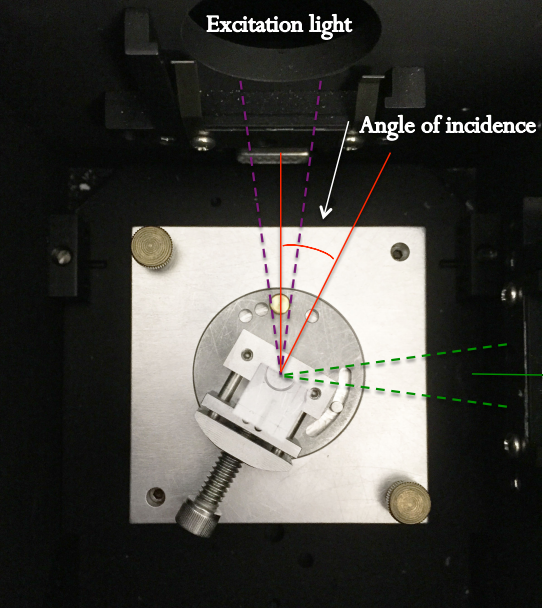
\includegraphics[width=200pt]{./figures/sample_placement.png}
	\label{fig:sample_placement}
\end{figure}

\section{Measurements} 
After irradiations, the samples showed coloration which partially disappeared after time due to the annealing of the substrate. 
The samples were repeatedly measured after irradiation until no additional annealing was seen. 
A typical fluorescence spectrum of EJ-200 is shown in Figure~\ref{fig:EJ200SP-1P-exc285}, 
after 3~Mrad at 9~krad/hr and after 3~Mrad at 429~krad/hr.

\begin{figure}[!htb]
	\centering
	\caption{Comparison between fluorescence spectrum of an irradiated sample to that of the non-irradiated sample excited at 285 nm.}
	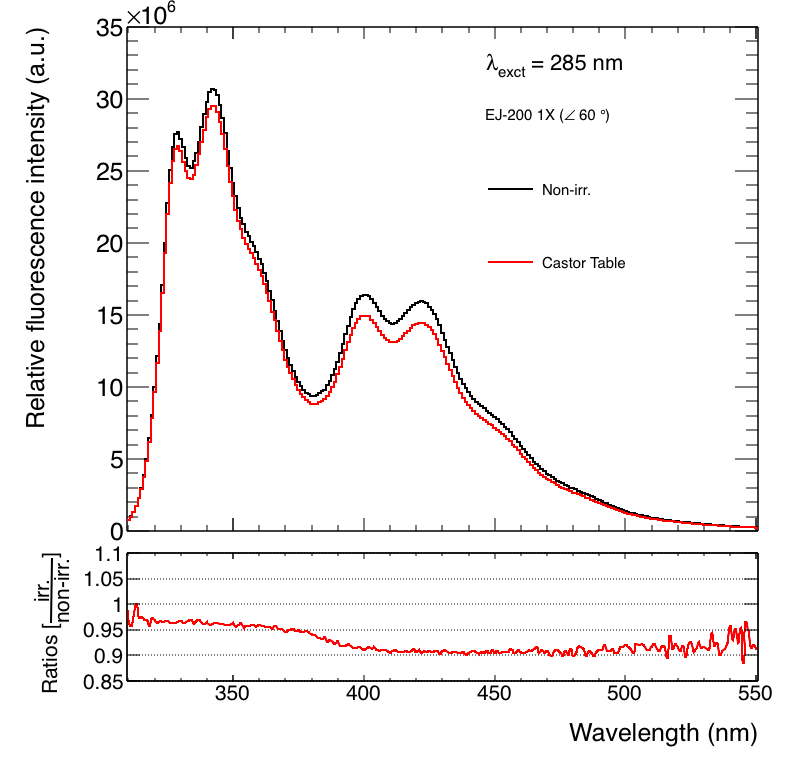
\includegraphics[width=300pt]{./figures/EJ200-1X-exc285.png}
	%%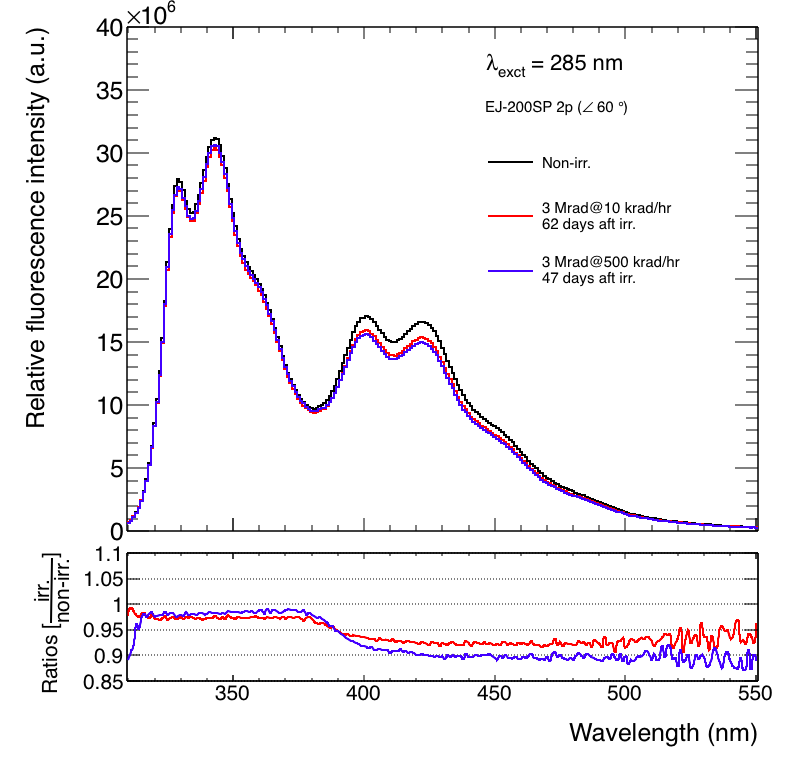
\includegraphics[width=175pt]{./figures/EJ200SP-2P-exc285.png}
	\label{fig:EJ200SP-1P-exc285}
\end{figure}

We calculate the light output ratio (R) using the integrated area of the irradiated sample's spectrum 
with respect to the corresponding non-irradiated one. 
Systematic uncertainties associated with the integrated area of each spectrum measurement are identified. 
Repeated measurements on the reference sample on different days, after turning off and on the instrument everyday, 
suggest the corresponding relative uncertainty to be $\pm$8\%. 
However, repeated measurements on the reference sample during the same day, when the spectrophotometer is continuously running, 
suggest the corresponding relative uncertainty to be $\pm$1\%. 
This indicates that although initialization conditions of the instrument strongly affect photon-counting, 
the instrument is stable after initialization.
Therefore the variation of intensity measured on different days is described by a normalization factor as a function of day, 
by measuring the reference sample. 
After correcting the integrated areas of spectra with their normalization factors, 
the uncertainty associated with instrument initialization is canceled in calculations of light yield ratios. 
Measurements on the reference sample when exciting its four different sides suggest the corresponding uncertainty to be $\pm$1\%, 
due to sample imperfection (optical surface, dopant concentration, etc). 
The monochromators have an accuracy of $\pm$0.5 nm, which translates into a negligible uncertainty on the integrated area of a spectrum. 
Since PMT's photon-counting obeys Poisson distribution and the number of photons is large, 
the corresponding random uncertainty is negligible. 
Therefore, due to mainly two independent uncertainties (sample imperfection and instrument systematic uncertainty), 
the uncertainty on light output ratio is found to be equal to or less than $\pm$2\%.

Table~\ref{table:1} shows light output ratios excited at three different wavelengths for 
1P and 2P samples of the same dose (3~Mrad) at different dose rates (9~krad/hr and 429~krad/hr). 
Table~\ref{table:2} shows light output ratios excited at three different wavelengths for 
1P and 2P samples of different doses at dose rate 9~krad/hr. 
Table~\ref{table:3} shows light output ratios excited at three different wavelengths for 
1X samples of same dose (6~Mrad) and dose rate (80~krad/hr), 
but at two different ambient temperatures (23~$^\circ$C and -30~$^\circ$C) during irradiation. 
Table~\ref{table:castor} shows light output ratios excited at three different wavelengths for 
1X and 2X samples of same dose (0.24~Mrad) at very low dose rate (0.24~krad/hr), 

\begin{table}[!ht]
\centering
  \caption{Light output ratios after irradiations of the same total dose and at different dose rates. The uncertainties on the total dose and dose rate are less than 2\%.}
  \begin{tabular}{c|c|c|c|c|c}
    \hline
    Sample		 &\begin{tabular}{@{}c@{}}Dose\\(Mrad)\end{tabular}  & \begin{tabular}{@{}c@{}}Dose rate \\(krad/hr)\end{tabular}  &$R_{285~nm}$	&$R_{350~nm}$	&$R_{400~nm}$	\\ \hline
    1P     	    	 & 2.95  	& 9.48 	 &0.95 ${\pm}$ 0.02 	&0.95 ${\pm}$ 0.02 	&0.92 ${\pm}$ 0.02 		\\ 
    1P			 & 2.95		& 429 	 &0.95 ${\pm}$ 0.02 	&0.91 ${\pm}$ 0.02 	&0.84 ${\pm}$ 0.02 		\\ \hline 
    2P     	    	 & 2.95  	& 9.48 	 &0.95 ${\pm}$ 0.02	&0.95 ${\pm}$ 0.02 	&0.92 ${\pm}$ 0.02 		\\ 
    2P			 & 2.95		& 429 	 &0.95 ${\pm}$ 0.02 	&0.91 ${\pm}$ 0.02 	&0.84 ${\pm}$ 0.02 		\\ \hline
  \end{tabular}
  \label{table:1}
\end{table}

\begin{table}[!ht]
\centering
  \caption{Light output ratios after irradiations of different total doses at dose rate 9 krad/hr. The uncertainties on the total dose and dose rate are less than 2\%.}
  \begin{tabular}{c|c|c|c|c|c}
    \hline
    Sample 		 &\begin{tabular}{@{}c@{}}Dose\\(Mrad)\end{tabular}  &\begin{tabular}{@{}c@{}}Dose rate \\(krad/hr)\end{tabular}  &$R_{285~nm}$	&$R_{350~nm}$	&$R_{400~nm}$	\\ \hline
    1P     	    	 & 2.95  	 &9.48 	 &0.95 ${\pm}$ 0.02	&0.95 ${\pm}$ 0.02 	&0.92 ${\pm}$ 0.02 		\\ 
    1P     	    	 & 4.00	   	 &9.20	 &0.93 ${\pm}$ 0.02 	&0.92 ${\pm}$ 0.02 	&0.87 ${\pm}$ 0.02 		\\ 
    1P			 & 6.95		 &9.32	 &0.90 ${\pm}$ 0.02 	&0.88 ${\pm}$ 0.02 	&0.81 ${\pm}$ 0.02 		\\ \hline
    2P     	    	 & 2.95	   	 &9.48	 &0.95 ${\pm}$ 0.02 	&0.95 ${\pm}$ 0.02 	&0.92 ${\pm}$ 0.02 		\\ 
    2P     	    	 & 4.00	   	 &9.20	 &0.94 ${\pm}$ 0.02 	&0.93 ${\pm}$ 0.02 	&0.90 ${\pm}$ 0.02 		\\ 
    2P			 & 6.95		 &9.32	 &0.90 ${\pm}$ 0.02 	&0.89 ${\pm}$ 0.02 	&0.83 ${\pm}$ 0.02 		\\ \hline
  \end{tabular}
  \label{table:2}
\end{table}

\begin{table}[!ht]
\centering
  \caption{Light output ratios after irradiation of 0.24~Mrad at 0.24~krad/hr. Note that the uncertainties on the total dose and dose rate are estimated to be 20\%.}
  \begin{tabular}{c|c|c|c|c|c}
    \hline
    Sample		 &\begin{tabular}{@{}c@{}}Dose\\(Mrad)\end{tabular}  & \begin{tabular}{@{}c@{}}Dose rate \\(krad/hr)\end{tabular}  &$R_{285~nm}$	&$R_{350~nm}$	&$R_{400~nm}$	\\ \hline
    1X     	    	 & 0.24 & 0.24  &0.94 ${\pm}$ 0.02&0.94 ${\pm}$ 0.02	&0.88 ${\pm}$ 0.02	\\ \hline 
    2X     	    	 & 0.24 & 0.24  &0.95 ${\pm}$ 0.02&0.97 ${\pm}$ 0.02	&0.90 ${\pm}$ 0.02	\\ \hline
  \end{tabular}
  \label{table:castor}
\end{table}

\begin{table}[!ht]
\centering
  \caption{Light output ratios after irradiations of the same total dose and dose rate at 23 $^\circ$C and -30 $^\circ$C.The uncertainties on the total dose and dose rate are less than 2\%.}
  \begin{tabular}{c|c|c|c|c|c}
    \hline
    Sample		 &\begin{tabular}{@{}c@{}}Dose\\(Mrad)\end{tabular}  &\begin{tabular}{@{}c@{}}Dose rate \\(krad/hr)\end{tabular}  &$R_{285~nm}$	&$R_{350~nm}$	&$R_{400~nm}$	\\ \hline
    1X, ~23 $^\circ$C	 & 5.82 	& 80.3 			 &0.90 ${\pm}$ 0.02	&0.88 ${\pm}$ 0.02	&0.77 ${\pm}$ 0.02		\\ 
    1X, -30 $^\circ$C	 & 5.82 	& 80.4 			 &0.90 ${\pm}$ 0.02	&0.84 ${\pm}$ 0.02	&0.70 ${\pm}$ 0.01		\\ \hline
  \end{tabular}
  \label{table:3}
\end{table}



\section{Interpretation}
Table~\ref{table:2} shows that radiation damage is not only to the base material, but also to the dopants of plastic scintillator. 
Measurements at 400~nm excitation wavelength, which almost exclusively excites the secondary dopant, 
show that the secondary dopant is increasingly damaged as the total dose increases. 

If the dose rate effect on light output is due to oxygen diffusion, then it is expected that the reduction in light output 
for the same dose would have a negative correlation with the dose rate, except for when the dose rate is low enough that 
oxygen permeates the entire sample. 
Comparing the light output ratios after irradiations of 3~Mrad dose at two different dose rates, 9~krad/hr and 429~krad/hr, 
we find no negative correlation between the reduction in light output and dose rate (Table~\ref{table:1}).
On the contrary, measurements at 400 nm excitation wavelength, which almost exclusively excites secondary dopant, 
show that the reduction in secondary dopant's light output is two times higher at 429~krad/hr than at 9~krad/hr.
Measurements at 350~nm excitation wavelength, which excites largely secondary dopant and non-negligible primary dopant, 
confirm greater reduction at 429~krad/hr in secondary dopant's light output. 
Measurements at 285~nm excitation wavelength, which excites PVT and primary dopant, show no significant difference 
in primary light output ratios between two dose rates. 

However, Table~\ref{table:castor} and Table~\ref{table:2} show that the amount of light output reduction is comparable 
between a total dose of 0.24~Mrad at very low dose rate 0.24~krad/hr and a total dose of 3-4~Mrad at a much higher dose rate 9~krad/hr.

The diffusion rate of oxygen in PVT is expected to be higher at higher temperature. 
Temperature also affects molecules' average kinetic energy and therefore various energy transfer mechanisms in the scintillator. 
Studies have shown temperature effects on plastic scintillator in pre-irradiation treatment~\cite{johnson} 
and post-irradiation annealing~\cite{birks1964}. 
However, there has been little study on the temperature effect during irradiation on plastic scintillators.
Table~\ref{table:3} suggests that more secondary dopant is damaged during the irradiation at -30~$^\circ$C than at 23~$^\circ$C.  

\section{Conclusion}
Using a fluorescence spectrophotometer, fluorescence emission output versus wavelengths for plastic scintillator EJ-200 with varying 
dopant concentrations is measured before and after irradiation for various doses and dose rates. 
Dose, dose rate, and temperature effects on the scintillator's dopants are investigated after irradiations.
We found that the plastic scintillator's secondary dopant is damaged by irradiation. 
This indicates that radiation damage is not only to the substrate but also to the dopants of plastic scintillators. 
Measurements of the light output from surface excitation show a dose rate effect in radiation damage to the secondary dopant, 
that the higher dose rate 429~krad/hr causes more damage to the secondary dopant than the lower dose rate 9~krad/hr. 
However, a total dose of 0.24~Mrad at very low dose rate 0.24~krad/hr causes the similar amount of damage to the dopants as 
a total dose of 3-4~Mrad at higher dose rate 9~krad/hr, suggesting nontrivial mechanisms of radiation damage to the dopants. 
In particular, sub-krad dose rate effect on scintillator light output is of interest to the upgrade of the CMS hadron calorimeter, 
and more comprehensive studies would help to better design hadron calorimeters and to better understand radiation damage on dopants.
We observe that more secondary dopant is damaged during the irradiation at -30~$^\citc$C than at 23~$^\circ$C. 
This is also of interest to the upgrade of the CMS hadron calorimeter, with the possible scenario of cold environment, 
which requires a deeper understanding of temperature effect on plastic scintillator during irradiation. 


%% The Appendices part is started with the command \appendix;
%% appendix sections are then done as normal sections
\appendix

\section{Absorption and Emission Spectra while Annealing}

Comparison between the variations in the bulk-material absorption spectrum and the fluorescence emission spectrum 
during the annealing process shows that significant change in the bulk absorption does not affect the fluorescence emission measurements. 

\begin{figure}[!ht]
	\centering
	\caption{Absorption spectra of irradiated samples (at 23~$^\circ$C and -30~$^\circ$C) repeatedly measured during the annealing process.}
	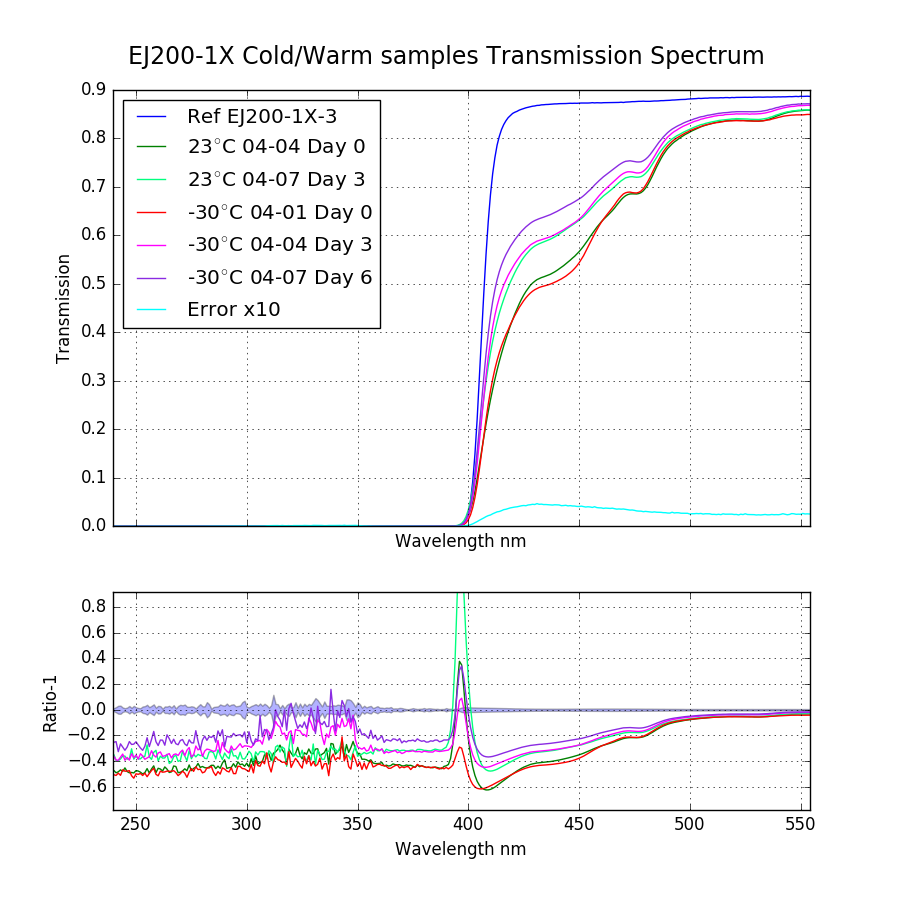
\includegraphics[width=300pt]{./figures/abs.png}
	\label{fig:abs}
\end{figure}

\begin{figure}[!ht]
	\centering
	\caption{Fluorescence spectra of the sample irradiated at 23$^\circ$C repeatedly measured during the annealing process.}
	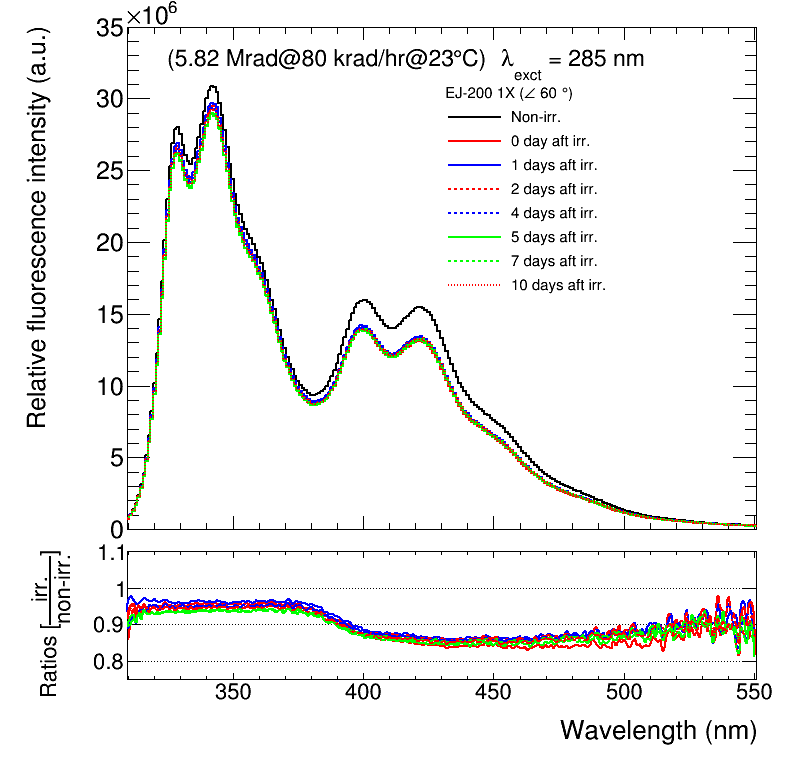
\includegraphics[width=300pt]{./figures/appendix1.png}
	\label{fig:app1}
\end{figure}

\begin{figure}[!ht]
	\centering
	\caption{Fluorescence spectra of the sample irradiated at -30$^\circ$C repeatedly measured during the annealing process.}
	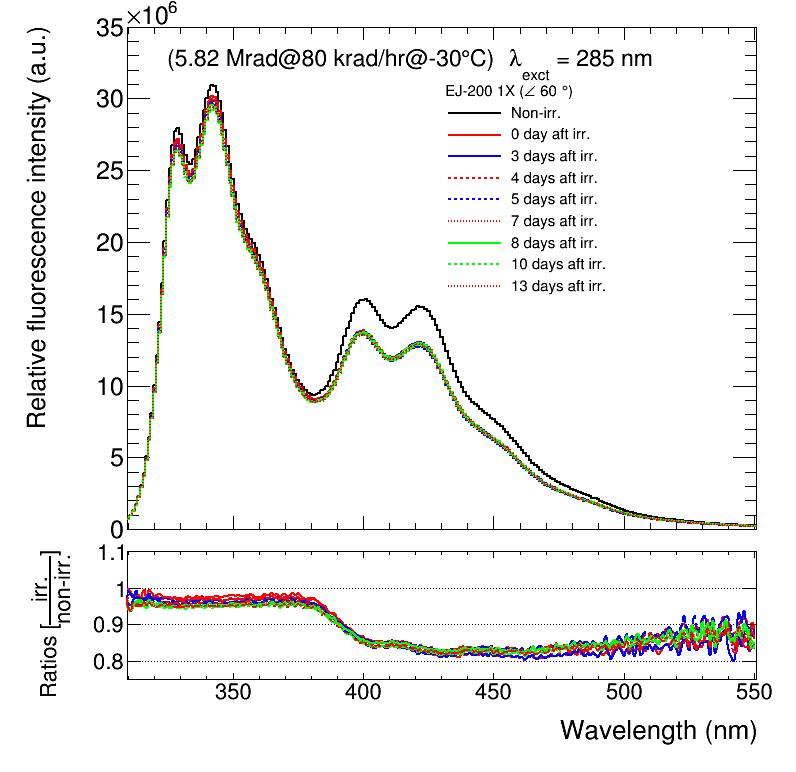
\includegraphics[width=300pt]{./figures/appendix2.png}
	\label{fig:app2}
\end{figure}

%% References
%%
%% Following citation commands can be used in the body text:
%% Usage of \cite is as follows:
%%   \cite{key}          ==>>  [#]
%%   \cite[chap. 2]{key} ==>>  [#, chap. 2]
%%   \citet{key}         ==>>  Author [#]

%% References with bibTeX database:

\bibliography{myBib}{}

%% Authors are advised to submit their bibtex database files. They are
%% requested to list a bibtex style file in the manuscript if they do
%% not want to use model1-num-names.bst.

%% References without bibTeX database:

% \begin{thebibliography}{00}

%% \bibitem must have the following form:
%%   \bibitem{key}...
%%

% \bibitem{}

% \end{thebibliography}


\end{document}

%%
%% End of file `elsarticle-template-1-num.tex'.
